\documentclass[12pt,a4paper,titlepage]{scrartcl}

\usepackage{comment}
\usepackage[main=ngerman,english]{babel}
\usepackage[utf8]{inputenc}
\usepackage[T1]{fontenc}
\usepackage{lmodern}
\usepackage{geometry}
\geometry{left=2.5cm,right=2.5cm,top=2.5cm,bottom=3cm,head=29pt,foot=25pt}
\setlength{\footheight}{25pt}
\usepackage{microtype}
\usepackage{amsmath,amssymb,mathtools}
\numberwithin{equation}{section}
\numberwithin{table}{section}
\numberwithin{figure}{section}
\usepackage{siunitx}
\sisetup{locale=US, separate-uncertainty=true, per-mode=fraction}
\usepackage{booktabs}
\usepackage{multirow}
\usepackage{graphicx}
\usepackage{float}
\usepackage{caption}
\usepackage{subcaption}
\usepackage[automark]{scrlayer-scrpage}
\usepackage[most]{tcolorbox}
\usepackage{hyperref}
\usepackage{pdfpages}
\usepackage{csvsimple-l3}
\usepackage{longtable}
\usepackage{graphicx}
\usepackage{mhchem}

%\input{../../jupyterpackages.tex}

% jupyter nbconvert --to latex 'Path'
% enferne usepackages und begin{document} und end{document}
% \input in main.tex mit \input{Path}


\newcommand{\pdfabbildung}[2]{%
    \refstepcounter{figure}%
    \addcontentsline{lof}{figure}{\protect\numberline{\thefigure}#1}%
    \label{#2}%
}

\newcommand{\pdftabelle}[2]{%
    \refstepcounter{table}%
    \addcontentsline{lot}{table}{\protect\numberline{\thetable}#1}%
    \label{#2}%
}


\hypersetup{colorlinks=true, linkcolor=blue!60!black, urlcolor=blue!60!black, citecolor=blue!60!black}

\clearpairofpagestyles

\chead{%
    \versuch\hfill\autor\\
    \rule{\textwidth}{0.2pt}%
}
\cfoot{%
    \rule{\textwidth}{0.2pt}\\[-0.5ex]
    \pagemark\ 
}
\addtokomafont{pagefoot}{\small}
\setlength{\parindent}{0pt}

\newtcolorbox{resultbox}[1][]{ 
    enhanced,
    colback=black!4!white,
    colframe=black!65!black,
    boxrule=0.8pt,
    arc=0.0mm,
    title=#1,
    fonttitle=\bfseries,
    %drop shadow
}


\newcommand{\versuch}{Versuch 21}
\newcommand{\titel}{Elektrolyse}
\newcommand{\praktikum}{Physikalisches Anfängerpraktikum 1}
\newcommand{\autor}{Jonathan Gießen}
\newcommand{\gruppe}{Gruppe 8}
\newcommand{\datum}{24. September 2026}
\newcommand{\betreuer}{Fabian Mrosek}

\begin{document}

\pagestyle{scrheadings}

\begin{titlepage}



    \centering
    \vspace*{4cm}
    {\large Universität Heidelberg\par}
    {\small Fakultät für Physik und Astronomie\par}
    {\Large \praktikum\par}
    \vspace{0.8cm}
    {\LARGE \bfseries \versuch\ -- \titel\par}
    \vspace{1.5cm}

    \begin{tabular}{ll}
        \textbf{Autor:} & \autor\\
        \textbf{Gruppe:} & \gruppe\\
        \textbf{Betreuer:} & \betreuer\\
        \textbf{Versuchsdatum:} & \datum\\
    \end{tabular}

    \vfill
    \hrulefill\
\end{titlepage}

\tableofcontents

\bigskip


\clearpage


\section{Einleitung}\label{sec:Einleitung}
Der Versuch 21 beschäftigt sich mit der Elektrolyse, einem chemischen Prozess, bei dem elektrische Energie genutzt wird, um eine chemische Reaktion zu erzwingen. Ziel des Versuchs ist es, die Grundlagen der Elektrolyse zu verstehen und die dabei auftretenden Phänomene zu beobachten und zu analysieren. Dabei wird die Faraday-Konstante experimentell bestimmt, die den Zusammenhang zwischen der Menge an elektrischer Ladung und der Menge an Stoff beschreibt, die bei der Elektrolyse umgesetzt wird.

\section{Grundlagen und Theorie}\label{sec:Grundlagen}
Lösungen von Säuren, Hydroxiden und Salzen und deren Schmelzen leiten den elektrischen Strom. Im Gegensatz zu den metallischen Leitern erfolgt der Ladungstransport aber nicht durch freie Elektronen sondern durch Ionen.
Befindet sich ein Elektrolyt im Feld zweier Elektroden, so tritt bei Stromfluss in der Regel eine Zersetzung des Elektrolytes auf. Man bezeichnet diesen Vorgang als Elektrolyse. \cite{PAPskript}

Die Faraday-Konstanet $F$ ist eine fundamentale physikalische Konstante, die den Zusammenhang zwischen der elektrischen Ladung und der Menge an Stoff beschreibt, die bei der Elektrolyse umgesetzt wird. 
Sie wird definiert:

\begin{equation}
    F = e \cdot N_A = \qty{9.648455(27)e4}{\coulomb\per\mol}
\end{equation}

Genau gesgt entpricht sie der Ladungsmenge, die durch einen Elektrolyten fließt, wenn sich 1/z Mol eines z-wertigenStoffes an der Elektrode absetzt. \cite{PAPskript}

Beim ersten Teil des Veruschs wird die Faraday-Konstante experimentell bestimmt, indem die Masse des abgeschiedenen Stoffes an der Elektrode gemessen wird, während eine bekannte elektrische Ladung durch den Elektrolyten fließt. Die Faraday-Konstante kann dann aus dem Verhältnis der abgeschiedenen Masse zur durchgeflossenen Ladung berechnet werden.

\begin{align}
    m &= n \cdot M_{Mol} = \frac{Q}{z \cdot F} \cdot M_{Mol} \\
    &\implies F = \frac{Q \cdot M_{Mol}}{z \cdot m} \label{eq:calc_masses}
\end{align}


Mit $m$ ist die Masse des abgeschiedenen Stoffes, $n$ die Stoffmenge, $M_{Mol}$ die molare Masse, $Q$ die durchgeflossene Ladung, $z$ die wertigkeit der Ionen und $F$ die Faraday-Konstante.

Um die Masse zu bestimmen, wird Kupfersulfat als Elektrolyt verwendet und der gemessene Masseverlust an der Anode und die Massezunahme an der Kathode verglichen. Die durchgeflossene Ladung wird durch die Messung des Stroms und der Zeit 9$Q = I \cdot t$ berechnet.

\begin{equation}
    \ce{CuSO4 <=> Cu^{2+} + SO4^{2-}}
\end{equation}

In zweiten Teil wird die Faraday-Konstante durch Elektrolyse von Wasser durch die Messung der abgeschiedenen Gasvolumina bestimmt. Dabei wird die Menge an Wasserstoff und Sauerstoff, die bei der Elektrolyse von Wasser entsteht, gemessen. Die Faraday-Konstante kann dann aus dem Verhältnis der abgeschiedenen Gasvolumina zur durchgeflossenen Ladung berechnet werden:

\begin{equation}
    n = \frac{Q}{z \cdot F} \implies F = \frac{Q}{z \cdot n}
\end{equation}

Die Stoffmenge $n$ beträgt

\begin{equation}
    n = \frac{V}{V_{Mol}}
\end{equation}
 
Das Molare Volumen $V_{Mol, 0}$ beträgt bei Normalbedingungen $\qty{22.414}{\liter\per\mol}$.

Um es auf die Bedingungen des Versuchs anzupassen, wird das Volumen auf die Normalbedingungen umgerechnet:

\begin{equation}
    V_{Mol} = \frac{p_0}{p} \cdot \frac{T}{T_0} \cdot V_{Mol,0}
\end{equation}

Mit $p_0 = \qty{1013.25}{\milli\bar}$, $T_0 = \qty{273.15}{\kelvin}$, $p$ dem gesamten Luftdruck und $T$ der Temperatur.

Der gesaamte Luftdruck $p$ setzt sich aus dem Umgebungsdruck $p_{L}$ und dem Sättigungsdampfdruck $P_{D}^{H_2SO_4}$ zusammen:
Näherungsweise entspricht der Dampfdruck der Schwefelsäure $p_D^{\ce{H2SO4}}$ 90\% des Dampfdrucks des Wassers $p_D^{\ce{H2O}}$

\begin{equation}
    p = p_L + p_D^{H_2SO4} = p_L + 0.9 \cdot p_D^{H_2O}
\end{equation}





    
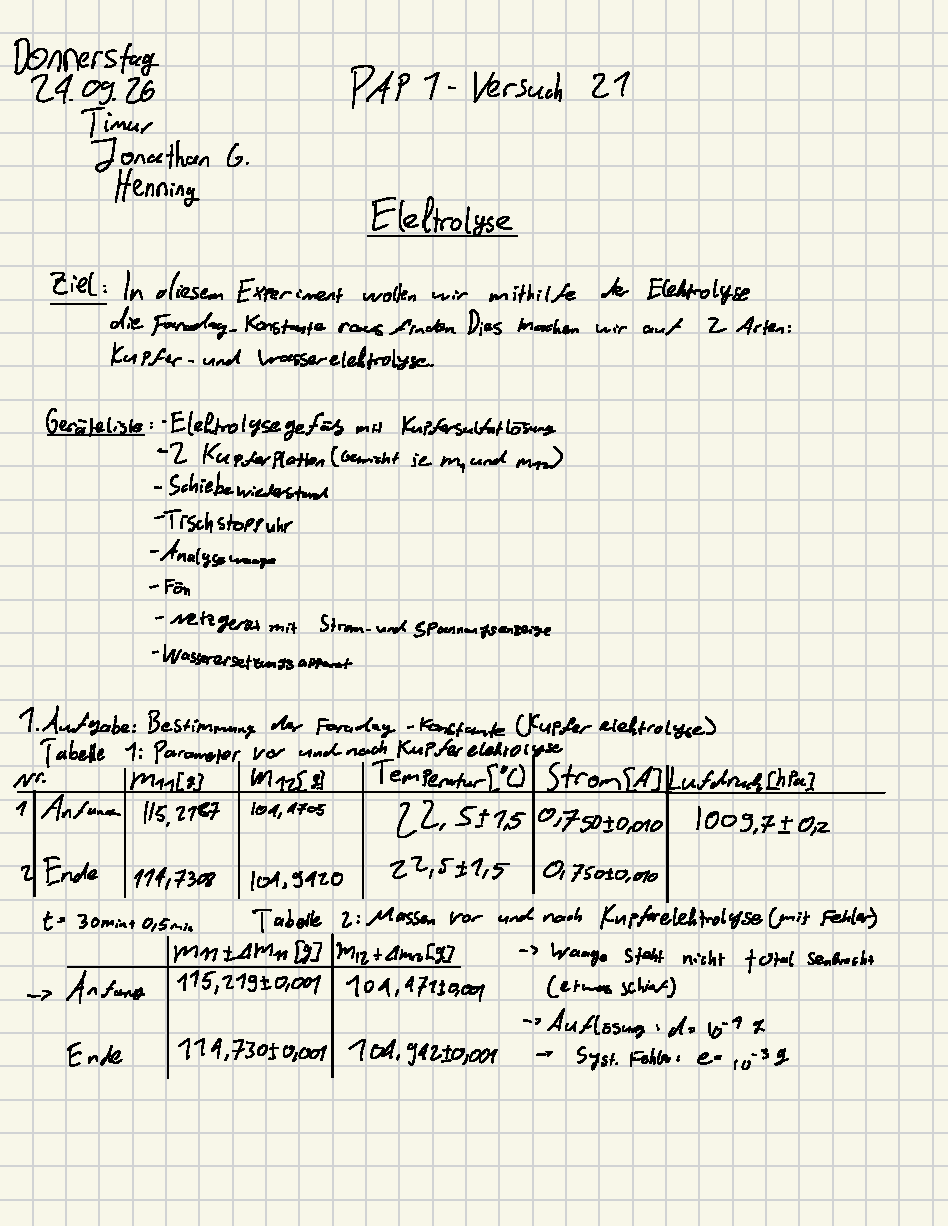
\includepdf[
    pages=-,
    width=\textwidth,
    height=0.95\textheight,
    keepaspectratio,
    pagecommand={\thispagestyle{scrheadings}},
    pagecommand*={\thispagestyle{scrheadings}\section{Messprotokoll}\subsection{Versuchsaufbau und Aufgaben}}
]{../Messprotokoll 21.pdf}


\subsection{Durchführung}

In diesem Versuch wird auf zwei Methoden die Faraday-Konstante bestimmt.

\paragraph{Teil 1}
Für 30 min wird ein konstanter Strom durch eine Kupfersulfatlösung geleitet. Dabei wird die Masse der Anode und Kathode vor und nach der Elektrolyse gemessen.

\paragraph{Teil 2}
In diesem Teil wird die Faraday-Konstante durch Elektrolyse von Wasser bestimmt. Es wird die Stromstärke und die Zeit gemessen, bis der Wasserstoff ein gewisses Volumen erreicht hat. Dabei wird die Temperatur und der Luftdruck gemessen, um das Volumen auf Normalbedingungen umzurechnen.


\section{Auswertung}

\subsection{Aufgabe 1: bestimmung der Faraday-Konstante durch Elektrolyse von Kupfersulfat}

An der Anode wird Kupfer oxidiert und geht in Lösung, während an der Kathode Kupfer reduziert wird und sich auf der Elektrode abscheidet. Die Masse der Anode nimmt ab, während die Masse der Kathode zunimmt.

\begin{align}
        &\text{Elektrolyt:} \quad \ce{&CuSO4 <=> Cu^{2+} + SO4^{2-}}\\
        &\text{Anode:} \quad \ce{&Cu(s) -> Cu^{2+} + 2e^-}\\
        &\text{Kathode:} \quad \ce{&Cu^{2+} + 2e^- -> Cu(s)}
\end{align}

Die Messwerte aus dem Messprotkoll betragen:

\begin{table}[H]

    \centering
    \caption{Messwerte für die Elektrolyse von Kupfersulfat.}
    \label{tab:messwerte_kupfersulfat}
    \begin{tabular}{lc}
        \toprule
        \textbf{Messwerte}\\
        \midrule
        Zeit des Stromflusses & $t = \qty{3600(30)}{\second}$ \\
        Stromstärke & $I = \qty{0.750(10)}{\ampere}$ \\
        Masse der Anode vor der Elektrolyse & $m_{Anode, vor} = \qty{115.2190(10)}{\milli\gram}$ \\
        Masse der Anode nach der Elektrolyse & $m_{Anode, nach} = \qty{114.7310(10)}{\milli\gram}$ \\
        Masse der Kathode vor der Elektrolyse & $m_{Kathode, vor} = \qty{104.4710(10)}{\milli\gram}$ \\
        Masse der Kathode nach der Elektrolyse & $m_{Kathode, nach} = \qty{104.9420(10)}{\milli\gram}$ \\
        \bottomrule
        \end{tabular}
\end{table}

Mit Gleichung \ref{eq:calc_masses} kann die Faraday-Konstante berechnet werden.
Die Fehlerformel beträgt:

\begin{equation}
    \Delta F = \sqrt{\left(\frac{t\cdot M_{Mol}}{z * m} \Delta I \right)^2 + \left(\frac{I\cdot M_{Mol}}{z * m} \Delta t\right)^2 + \left(\frac{I\cdot t\cdot M_{Mol}}{z * m^2} \Delta m\right)^2}
\end{equation}





\clearpage

\listoffigures


\listoftables

\begin{thebibliography}{5}
    \bibitem{PAPskript} Dr. J.Wagner, \emph{Physikalisches Anfängerpraktikum}, Stand 11/2024
    \bibitem{ilberg1988physikalisches} W. Ilberg, M. Krötzsch, \emph{Physikalisches Praktikum für Anfänger}, BSB B. G. Teubner Verlagsgesellschaft, Leipzig (1985).
\end{thebibliography}




\begin{comment}

\begin{table}[H]
    \centering
    \caption{Mess- und Geräteparameter für die exemplarische Berechnung (Messung 28).}
    \label{tab:parameter_messung_28}
    \begin{tabular}{ll}
        \toprule
        \textbf{Größe} & \textbf{Wert} \\
        \midrule
        Fallstrecke & $s_1 = 10\,\text{Skt} = 5.00 \cdot 10^{-4}\,\text{m}$ \\
        Fallzeit & $t_1 = 11.85\,\text{s}$ \\
        Steigstrecke & $s_2 = 10\,\text{Skt} = 5.00 \cdot 10^{-4}\,\text{m}$ \\
        Steigzeit & $t_2 = 18.19\,\text{s}$ \\
        Skalenteilung & $1\,\text{Skt} = 5.00 \cdot 10^{-5}\,\text{m}$ \\
        Kondensatorspannung & $U = 500\,\text{V}$ \\
        Plattenabstand & $d = 6.00 \cdot 10^{-3}\,\text{m}$ \\
        Luftdruck & $p = 100285\,\text{Pa}$ \\
        Erdbeschleunigung & $g = 9.81\,\frac{\text{m}}{\text{s}^2}$ \\
        Dichtedifferenz & $\rho = \rho_{\text{Öl}} - \rho_{\text{Luft}} = 871.21\,\frac{\text{kg}}{\text{m}^3}$ \\
        Unkorrigierte Luftviskosität & $\eta_0 = 1.81 \cdot 10^{-5}\,\text{Pa}\cdot\text{s}$ \\
        Cunningham-Konstante & $b = 7.78 \cdot 10^{-3}\,\text{Pa}\cdot\text{m}$ \\
        \bottomrule
    \end{tabular}
\end{table}
\end{comment}
\end{document}